\chapter{Experimental Apparatus}
\label{chap:experiment}

What machines must we build to examine the smallest pieces of the universe? The famous equation 
$E = m$ provides that to create massive particles, we need to provide enough energy. In order to give 
kinematic phase space to the types of processes that are examined in this thesis (and many others besides),
a system must be created in which there is enough energy to (at bare minimum), overcome kinematic thresholds:
if you want to search for $HH$ decays, you should have at least \SI{250}{\GeV} ($= 2\times m_{H}$) to work with.
It is not enough to simply induce such processes, however. These processes need to be captured in some way, emitted 
energy and particles must be characterized and identified, and in the end all of this information must be put into a 
useful and useable form such that selections can be made, statistics can be run, and a meaningful statement 
can be made about the universe. In this chapter, we describe the machines behind the physics, namely the Large 
Hadron Collider and the ATLAS experiment.

\section{The Large Hadron Collider}
The Large Hadron Collider is a particle accelerator near Geneva, Switzerland. In broad scope, it is a 
ring with a 27 kilometer circumference. Hadrons (usually protons or heavy ions) move in two 
counter-circulating beams, which are made to collide at four collision points at various 
points on the ring. These four collision points correspond to the four detectors placed 
around the ring: two ``general purpose'' experiments: ATLAS and CMS; LHCb, focused primarily 
on flavor physics; and ALICE, focused primarily on heavy ions.

The focus of this thesis is proton-proton collisions at center of mass energy $\sqrt{s}=\SI{13}{\TeV}$. 
The process to achieve such collisions proceeds as follows:
first, an electric field strips hydrogen of its electrons, creating protons. A linear accelerator,
LINAC 2, accelerates protons to \SI{50}{\MeV}. The resulting beam is injected into the Proton 
Synchrotron Booster (PSB), which pushes the protons to \SI{1.4}{\GeV}, and then the Proton Synchrotron,
which brings the beam to \SI{25}{\GeV}.

Protons are then transferred to the Super Proton Synchrotron (SPS), which ramps up the energy to 
\SI{450}{\GeV}. Finally, the protons enter the LHC itself, bringing the beam up to \SI{6.5}{\TeV}. \todo{cite: https://home.cern/science/accelerators/accelerator-complex}

While there is, of course, much that goes into the Large Hadron Collider development and operation, perhaps
two of the most fundamental ideas are (1) how are the beams directed and manipulated and (2) what do we 
mean when we say ``protons are accelerated''. These questions both are directly answered by pieces of hardware,
namely (1) magnets and (2) radiofrequency (RF) cavities.

One of fundamental components of the LHC is a large set of superconducting niobium-titanium magnets. These 
are cooled by liquid helium to achieve superconducting temperatures, and there are several types with very 
specific purposes. The obvious first question with a circular accelerator is how to keep the particle beam 
moving around in that circle. This job is done via a set of dipole magnets placed around the \emph{beam pipes}: the 
tubes containing the beam. These are designed such that the magnetic field in the center of the beam pipe runs 
perpendicular to the velocity of the charged particles, providing the necessary centripetal force for 
the synchrotron motion.

A proton beam is not made of a single proton, however, but of many protons, grouped into a series of \emph{bunches}.
As all of these are positively charged, if unchecked, these bunches would become diffuse and break apart. What we 
want is a stable beam with tightly clustered protons to maximize the chance of a high energy collision.
Such clustering is done via a series of quadropole magnets, with field distributed as in 
\todo{grab image from General Exam}. Alternating sets of quadropoles provide the necessary forces for a tight, 
stable beam. While these are the two major components of the LHC magnet system, it is not the full story -- higher order 
magnets are used to correct for small imperfections in the beam \todo{expand}.

Magnetic fields do no work, however, so the magnet system is unable to do the job of the actual acceleration. This is 
accomplished via a set of radiofrequency (RF) cavities. Within these cavities, an electric field is made to 
oscillate (switch direction) at a precise rate. These rates interact with the beam via in RF \emph{buckets}, with 
bunches corresponding to groups of protons that fill a given bucket. The timing is such that protons will always 
experience an accelerating voltage, corresponding to the \SI{25}{\ns} bunch spacing used at the LHC.

A nice property of this bucket/bunch configuration is that there is some self-correction -- there is 
some finite spread in the grouping of particles. If a particle arrives too early, it will experience some 
decelerating voltage; if too late, it will experience a higher accelerating voltage.

\subsection{The LHC Schedule}
The physics program at the Large Hadron Collider is split into a variety of data taking periods called \emph{runs}.
these runs correspond to various detector/accelerator configurations, and are interspersed with \emph{long shutdowns} -- 
periods used for detector/accelerator upgrades in preparation for the next run. The LHC timeline is as follows 
\begin{enumerate}
	\item Run 1 (2010--2013): First run of the LHC, operating at center of mass energy $\sqrt{s}=\SI{7}{\TeV}$, 
	increased to \SI{8}{\TeV} in 2012. ATLAS recorded \SI{4.57}{\ifb} and \SI{20.3}{\ifb} of data usable for physics
	at $\sqrt{s}=$\SI{7}{\TeV} and \SI{8}{\TeV} respectively.
	\item Long Shutdown 1 (LS1; 2013--2015): Upgrades to accelerator complex, magnet system, to allow for increase 
	in energy. Design energy was $\sqrt{s}=\SI{14}{\TeV}$, delays in ``training'' of superconducting magnets 
	led to decrease to $\sqrt{s}=\SI{13}{\TeV}$.
	\item Run 2 (2015--2018): Second run of the LHC, operating at center of mass energy $\sqrt{s}=\SI{13}{\TeV}$. 
	Data from this run is used in this thesis, with \SI{139}{\ifb} of data available for physics from the ATLAS
	experiment.
	\item Long Shutdown 2 (LS2; 2019--2021): Upgrades to ATLAS muon spectrometer (New Small Wheel), liquid argon 
	calorimeter; upgrades in preparation for the High Luminosity LHC (HL-LHC).
	\item Run 3 (2021--2023?): Third run of the LHC, target center of mass energy $\sqrt{s}=13-\SI{14}{\TeV}$, 
	total target luminosity \SI{300}{\ifb}.
	\item Long Shutdown 3 (LS3; 2024?--2026?): Further upgrades for the HL-LHC.
	\item Run 4, 5, \ldots ? (2026? onward): High Luminosity LHC -- goal is to achieve instantaneous luminosities 
	by a factor of five, massively enlarging available statistics for physics. Projected 3000 to \SI{4000}{\ifb}, 
	$> 20$ times the full Run 2 ATLAS dataset.
\end{enumerate}


\section{The ATLAS Experiment}
\label{sec:ATLAS}

\begin{figure}[ht]
\centering
\subfloat{
		  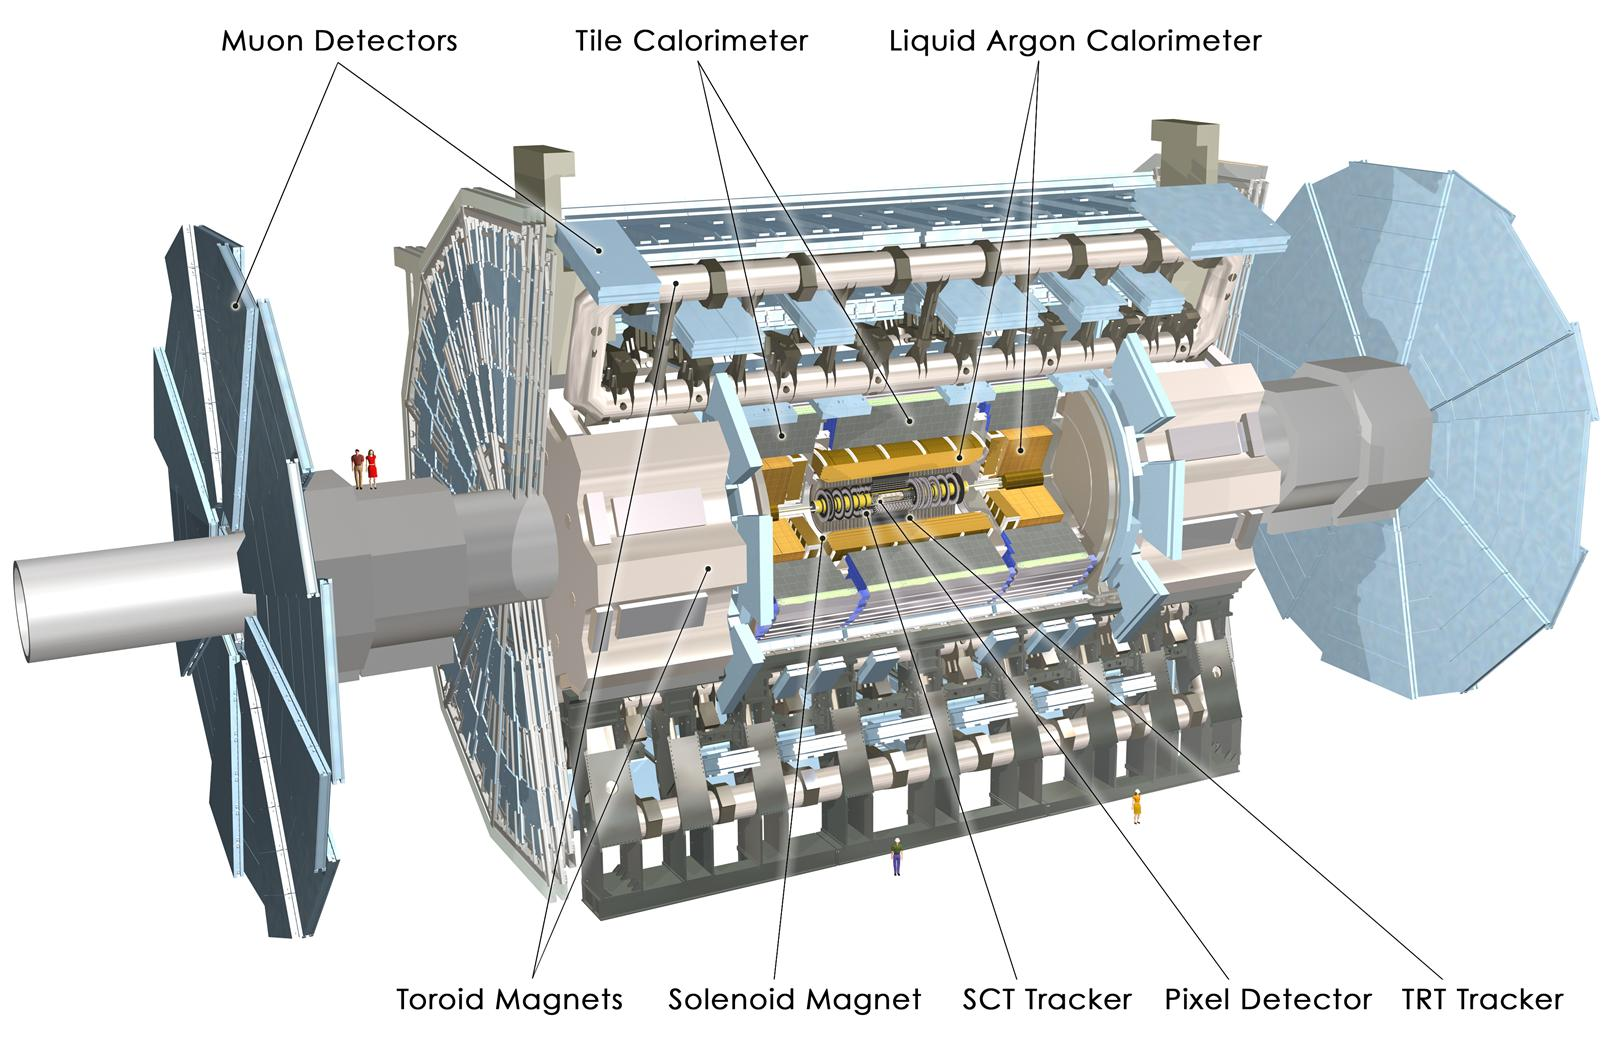
\includegraphics[width=0.8\textwidth]{figures/ATLAS-det.jpeg}
		 }
\caption{Diagram of the ATLAS detector \cite{DetectorImage} \label{fig:ATLAS-det}}
\end{figure}

This thesis focuses on searches done with the ATLAS experiment. As mentioned, this is 
one of two ``general purpose'' experiments at the LHC, by which we mean there is a 
very large and broad variety of physics done within the experimental collaboration. 
This broad physics focus has a direct relation to the design of the ATLAS detector~\cite{PERF-2007-01}, pictured 
in Figure \ref{fig:ATLAS-det}, which is composed of a sophisticated set of subsystems designed 
to fully characterize the physics of a given high energy particle collision. It consists of an inner 
tracking detector surrounded by a thin superconducting solenoid, electromagnetic and hadronic calorimeters,
and a muon spectrometer incorporating three large superconducting toroidal magnets. The ATLAS detector 
covers nearly the entire solid angle around the collision point, fully characterizing the ``visible'' 
components of a collision and allowing for indirect sensitivity to particles that do not interact with the detector 
(e.g. neutrinos) via ``missing'' energy (roughly momentum balance). We will go through the design and physics 
contribution of each of the detector components in the following. A schematic of how various particles 
interact with the detector is shown in Figure \ref{fig:ATLAS-shower}.

\begin{figure}[ht]
\centering
\subfloat{
		  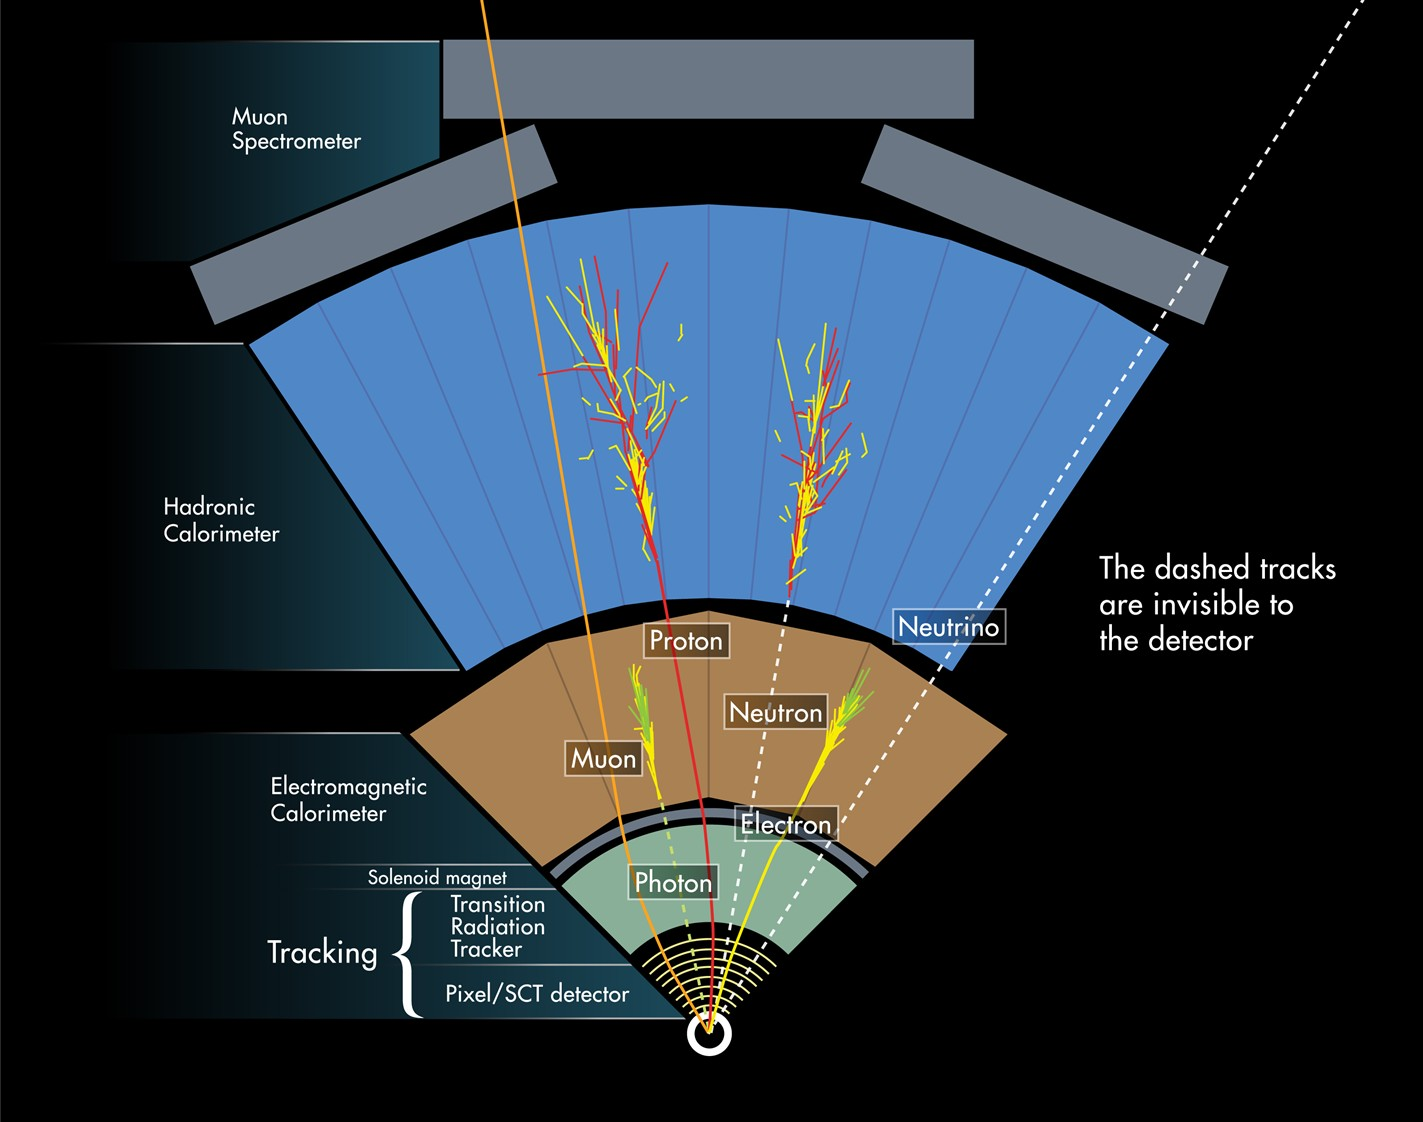
\includegraphics[width=0.8\textwidth]{figures/ATLAS-shower.jpeg}
		 }
\caption{Cross section of the ATLAS detector showing how particles interact with various detector components \cite{ShowerImage} \label{fig:ATLAS-shower}}
\end{figure}

\subsection{ATLAS Coordinate System} 
\begin{figure}[ht]
\centering
\subfloat{
		  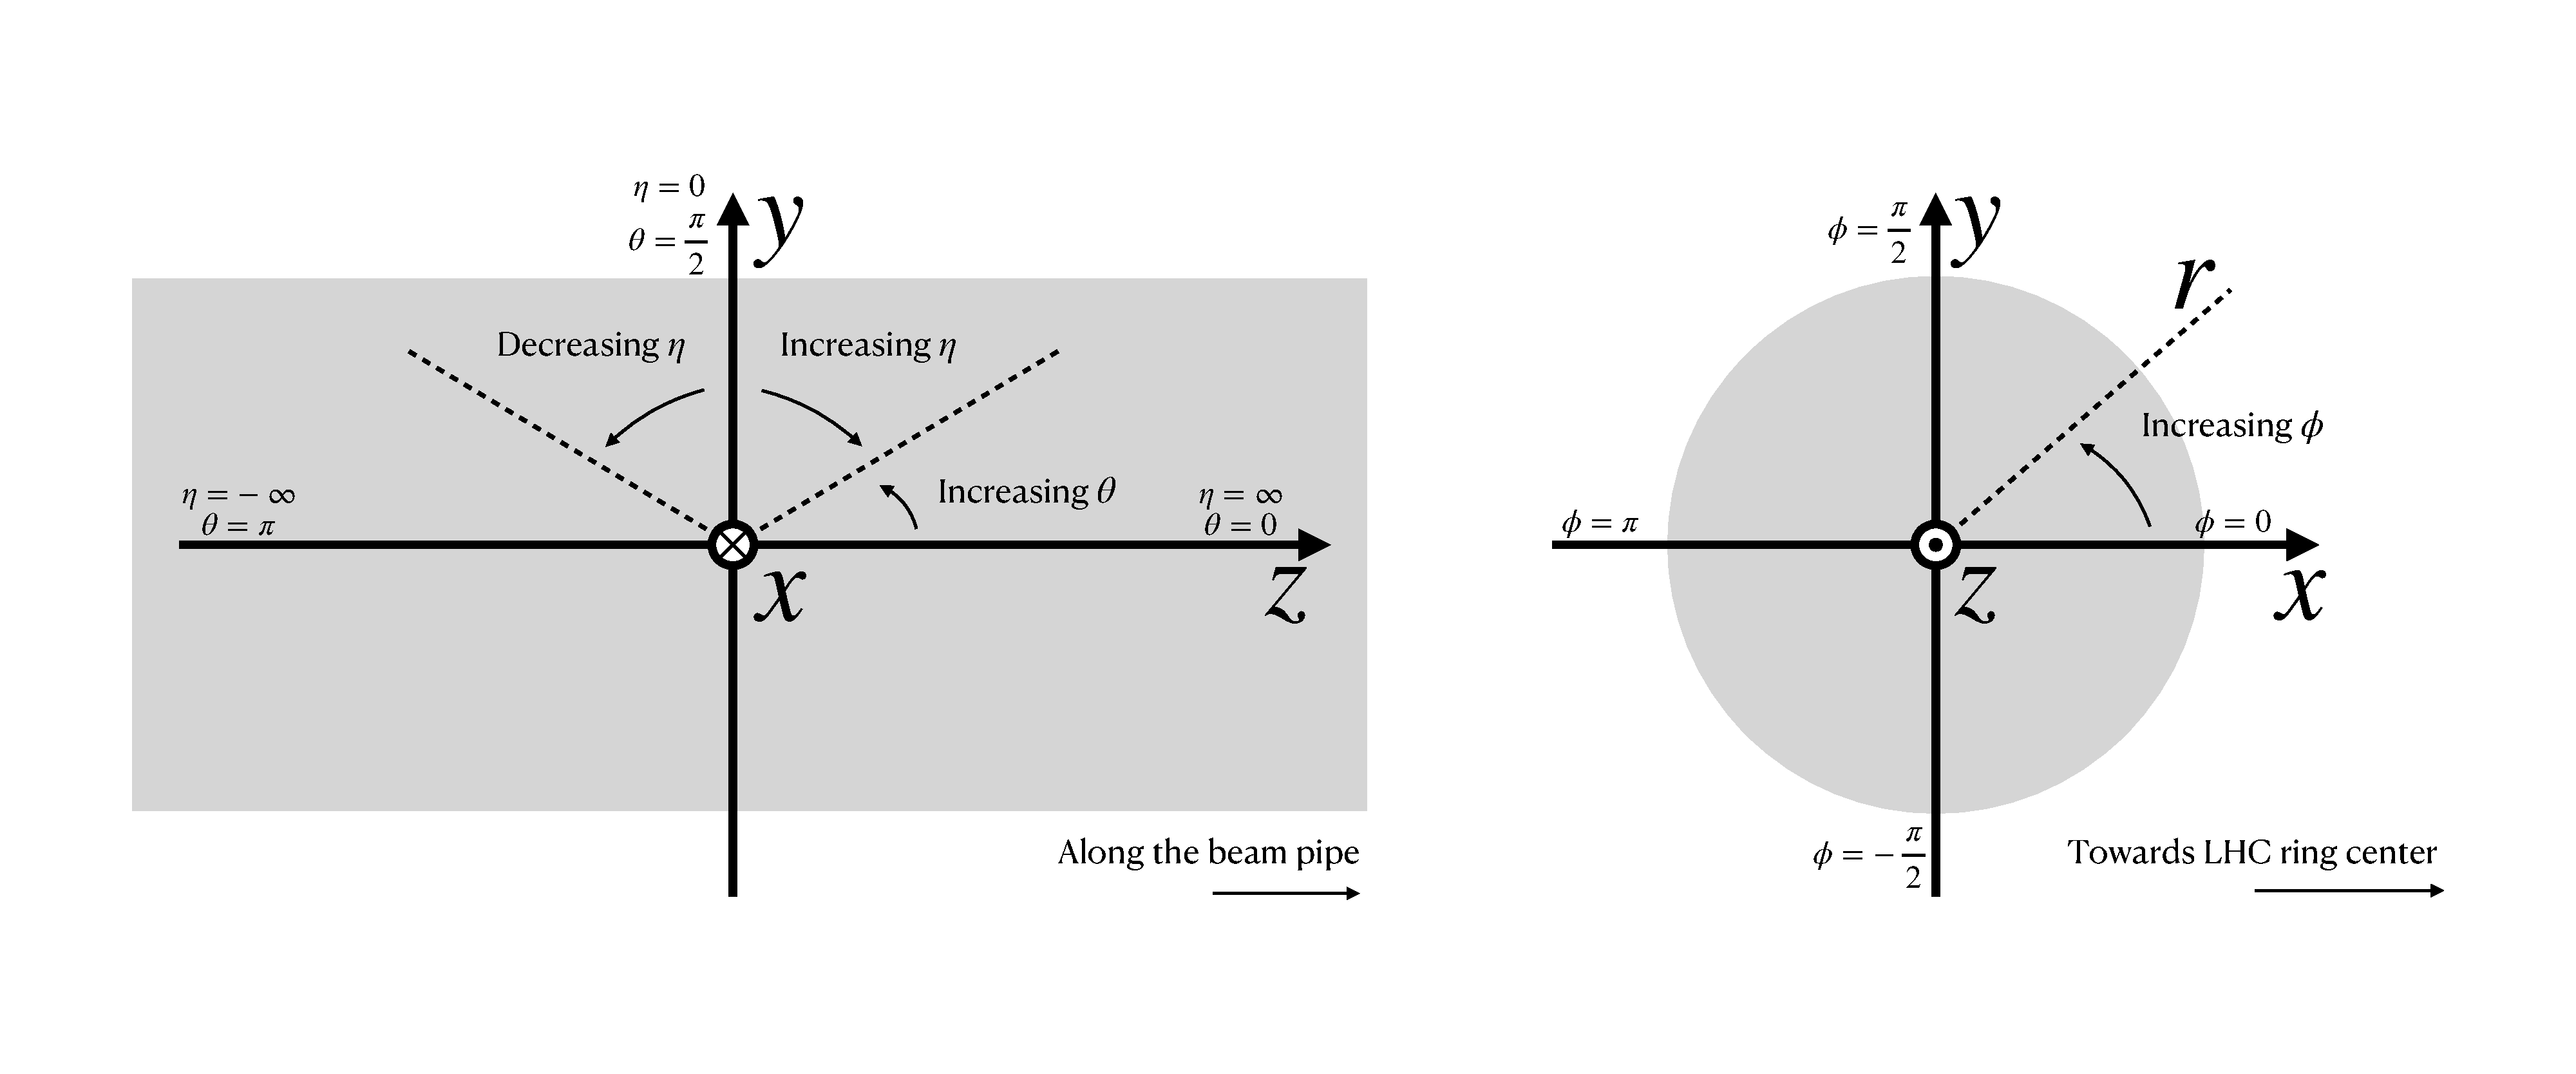
\includegraphics[width=1.0\textwidth]{figures/ATLAS-coords.pdf}
		 }
\caption{2D projections of the ATLAS coordinate system\label{fig:ATLAS-coords}}
\end{figure}

Of relevance for the following discussion, as well as for the analysis presented in Chapter \ref{chap:bbbb},
is the ATLAS coordinate system. ATLAS uses a right-handed coordinate system with its origin at the nominal 
interaction point (IP) in the center of the detector and the \(z\)-axis along the beam pipe.
The \(x\)-axis points from the IP to the centre of the LHC ring, and the \(y\)-axis points upwards.
Cylindrical coordinates \((r,\phi)\) are used in the transverse plane, \(\phi\) being the azimuthal angle 
around the \(z\)-axis. The pseudorapidity is defined in terms of the polar angle \(\theta\) as 
\(\eta = -\ln \tan(\theta/2)\). Angular distance is measured in units of 
\(\Delta R \equiv \sqrt{(\Delta\eta)^{2} + (\Delta\phi)^{2}}\). These coordinates are shown in Figure 
\ref{fig:ATLAS-coords}.

\subsection{Inner Detector}
The purpose of the inner detector is the reconstruction of the trajectory of charged particles, called 
\emph{tracking}. This is accomplished primarily through the collection of electrons displaced when a 
charged particle passes through a tracking detector. By setting up multiple layers of such detectors, 
such that a given particle leaves a signature, known as a``hit'', in each layer, the trajectory of 
the particle may be inferred via ``connecting the dots'' between these hits.

The raw trajectory of a particle only provides positional information. However, the trajectory 
of a charged particle in a known magnetic field additionally provides information on particle 
momentum and charge via the curvature of the corresponding track (cf. $\vec{F} = q\vec{v}\times \vec{B}$).
The inner detector system is therefore surrounded by a solenoid magnet, providing a \SI{2}{\tesla} magnetic 
field along the $z$-axis (yielding curvature in the transverse $x-y$ plane).

The inner detector provides charged particle tracking in the range \(|\eta| < 2.5\) via a series of 
detector layers. The innermost of these is
the high-granularity silicon pixel detector which typically provides four measurements per track, with the 
first hit in the insertable B-layer (IBL) installed before Run~2~\cite{ATLAS-TDR-19,PIX-2018-001}. This 
is very close to the interaction point with a high degree of positional information, and is therefore 
very important for e.g. $b$-tagging (see Chapter \ref{chap:reconstruction}). It is followed by the silicon 
microstrip tracker (SCT), which usually provides eight measurements per track. This is lower granularity, but 
similar in concept to the pixel detector.

Both of these silicon detectors are complemented by the transition radiation tracker (TRT),
which extends the radial track reconstruction within the range \(|\eta| < 2.0\). This is a different 
design, composed of \emph{drift tubes}, i.e. straws filled with Xenon gas with a wire in the center, 
but similarly collects electrons displaced by ionizing particles. In addition, the TRT includes materials 
with widely varying indices of refraction, which leads to the production of transition radiation, namely 
radiation produced by a charged particle passing through an inhomogeneous medium. The energy loss on 
such a transition is proportional to the Lorentz factor $\gamma = E/m$ -- correspondingly, lighter 
particles (e.g. electrons) tend to lose more energy and emit more photons compared to heavier particles 
(e.g. pions). In the detector, this corresponds to a larger fraction of hits (typically 30 in total) above a 
given high energy-deposit threshold for electrons, providing particle identification information.

\subsection{Calorimeter}
Surrounding the inner detector in ATLAS is the calorimeter. The principle of the calorimeter is to 
completely absorb the energy of a produced particle in order to measure it. However, a pure block 
of absorber does not provide much information about the particle interaction with the material. 
The ATLAS calorimeter therefore has a \emph{sampling calorimeter} structure, namely, layers 
of absorber interspersed with layers of sensitive material, giving the calorimeter ``stopping power'' 
while allowing detailed measurement of the resulting particle shower and corresponding deposited energy.

The ATLAS calorimetersystem covers the pseudorapidity range \(|\eta| < 4.9\), 
and is primarily composed of two components, an electromagnetic calorimeter, 
designed to measure particles which primarily interact via electromagnetism 
(e.g. photons and electrons), and a hadronic calorimeter, designed to measure 
particles which interact via the strong force (e.g. pions, other hadrons). We 
will return to the differences between these in a moment. 

In ATLAS, the electromagnetic calorimeter covers the region of \(|\eta|< 3.2\),
and uses lead for the absorbers and liquid-argon for the sensitive material. It is high 
granularity and, geometrically, has two components: the ``barrel'', which covers the cylindrical body 
of the detector volume and the ``endcap'', covering the ends. An additional thin liquid-argon presampler 
covers \(|\eta| < 1.8\) to correct for energy loss in material upstream of the calorimeters.

The hadronic calorimeter is composed of alternating steel and plastic scintillator tiles,
segmented into three barrel structures within \(|\eta| < 1.7\), in addition to two copper/liquid-argon 
endcap calorimeters.

The solid angle coverage is completed with forward copper/liquid-argon and tungsten/liquid-argon 
calorimeter modules optimized for electromagnetic and hadronic energy measurements respectively.

\subsection{Muon Spectrometer}
While muons interact electromagnetically, they are around 200 times heavier than electrons 
($m_{\mu}$ = \SI{106}{\MeV}, while $m_{e}$ = \SI{0.510}{\MeV}. 
Therefore, electromagnetic interactions with absorbers in the calorimeter 
are not sufficient to stop them, and, as they do not interact via the strong force, hard scattering with 
nuclei is rare. A dedicated system for muon measurements is therefore required. 

The muon spectrometer (MS) is the outermost layer of ATLAS and is designed for this purpose. It is composed 
of three parts: a set of triggering chambers, which detect if there is a muon and provide 
a coordiate meaurement, in conjunction with high-precision tracking chambers, which measure the deflection of 
muons in a magnetic field to measure muon momentum, similar to the inner detector solenoid. The magnetic 
field is generated by the superconducting air-core toroidal magnets, with a field integral between 
\num{2.0} and \SI{6.0}{\tesla\metre} across most of the detector. The toroid magnetic field runs roughly 
in a circle in the $x-y$ plane around the beam line, leading to muon curvature along the z-axis.

The precision tracking system covers the region \(|\eta| < 2.7\) via three layers of monitored drift 
tubes, and is complemented by cathode-strip chambers in the forward region, where the background is highest.
The muon trigger system covers the range \(|\eta| < 2.4\) with resistive-plate chambers in the barrel, and thin-gap chambers in the endcap regions.

\subsection{Triggering}
During a typical run of the LHC, there are roughly 1 billion collisions in ATLAS per second (\SI{1}{\GHz}), corresponding
to a \SI{40}{\MHz} bunch crossing rate. 
\todo{cite: https://cds.cern.ch/record/1457044/files/ATLAS\%20fact\%20sheet.pdf}
Saving the information from all of them is not only unnecessary, but infeasible. The ATLAS trigger 
system provides a sophisticated set of selections to filter the collision data and only keep those 
collision events useful for downstream analysis.

These events are selected by the first-level trigger system, which is implemented in custom hardware,
and accepts events at a rate below \SI{100}{\kHz}. Selections are then made by algorithms implemented in software 
in the high-level trigger~\cite{TRIG-2016-01}, reducing this further, and, in the end, events 
are recorded to disk at much more manageable rate of about \SI{1}{\kHz}.

An extensive set of ATLAS software~\cite{ATL-SOFT-PUB-2021-001} is open source, including the software used for real and simulated data reconstruction and analysis and that used in the trigger and data acquisition systems of the experiment.

\subsection{Particle Showers and the Calorimeter}
The design of the ATLAS detector is directly tied to the physics it is trying to detect. Of these, 
possibly the most non-trival distinction is in the calorimeter design. It is therefore useful to discuss in more 
detail the various properties of electromagnetic and hadronic interactions with material, and how these 
correspond to the particle showers measured by the detector described above. 

Electromagnetic showers in ATLAS predominantly occur via bremsstrahlung, or ``braking radiation'', and electron-positron 
pair production. This proceeds rougly as follows: an electron entering a material is deflected by the electromagnetic 
field of a heavy nucleus. This results in the radiation of a photon. That photon produces an electron-positron 
pair, and the process repeats, resulting in a shower structure. At each step, characterized by 
\emph{radiation length}, $X_{0}$, the number of particles approximately doubles and the average particle 
energy decreases by approximately a factor of two. \todo{Include nice Thomson image}

Note that bremsstrahlung and pair production only dominate in specific energy regimes, with other processes 
taking over depending on particle energy. For electrons, bremsstrahlung only dominates for higher energies,  
as low energy electrons will form ions with the atoms of the material. The point where the rates for the 
two processes are equal is called the \emph{critical energy}, and is roughly
\begin{equation}
E_{c} \approx \frac{\SI{800}{\MeV}}{Z}
\end{equation}
where $Z$ is the nuclear charge. From a similar analysis of rates, we may see that the bremsstrahlung 
rate is inversely proportional to the square of the mass of the particle. This explains why muons do not 
shower in a similar way, as the rate of bremsstrahlung is suppressed by $(m_{e}/m_{\mu})^2$ relative to electrons.

For lead, the absorber used for the ATLAS electromagnetic calorimeter, which has $Z=82$, this critical energy 
is therefore around \SI{10}{\MeV}. Electrons resulting from LHC collisions are of a $\SI{}{\GeV}$ scale. 
With the approximation of a reduction in particle energy by a factor of two every radiation length, the number of radiation lengths before the critical energy is reached is 
\begin{equation}
x = \frac{\ln{(E/E_{c})}}{\ln{2}}
\end{equation}
such that for a \SI{100}{\GeV} shower in lead, $x\sim 13$. The radiation length for lead is around \SI{0.56}{\cm},
such that an electromagnetic shower could be expected to be captured within \SI{10}{\cm} of lead. 

Electromagnetic showers are therefore characterized by depositing much of their energy within a small region 
of space. As we show below (Chapter \ref{chap:simulation}) though electromagnetic showering is not deterministic, 
the large number of particles and the restricted set of processes involved means that the shower development as a whole 
is very similar between individual electromagnetic showers of the same energy.

For completeness, note as well that pair production dominates for photons of energy greater than around \SI{10}{\MeV}, 
whereas for lower energies (below around \SI{1}{\MeV}), the photoelectric effect, namely atomic photon absorption and electron emission, dominates.

Hadronic showers are distinguished by the fact that they interact strongly with atomic nuclei. They are 
correspondingly more complex because (1) they involve a wider variety of processes than electromagnetic 
showers, and (2) these processes have a wide variety of associated length scales. Because these are 
heavier than electrons (e.g. protons and charged pions) bremsstrahlung is suppressed, but ionization interactions 
with the electrons will cause these particles to lose energy as they pass through the material. Hadronic 
showering occurs on interaction with atomic nuclei. This may lead to production of, e.g. both charged ($\pi^{\pm}$)
and neutral ($\pi^{0}$) pions. The $\pi^{0}$ lifetime is much much shorter than that of the charged pions (around 
a factor of $10^8$), and immediately decays to two photons, starting an electromagnetic shower, as described 
above. The longer lived $\pi^{\pm}$ travel further in the detector before experiencing another strong interaction 
with more particles produced, also with varying lifetimes and decay properties. 

It is therefore immediately apparent that hadronic showers are more complex than electromagnetic ones 
(electromagnetic showers can be a subset of the hadronic!), and therefore much more variable from shower 
to shower. The length scales involved are also significantly larger due to the reliance on nuclear interactions,
characterized by length $\lambda_{I}$, which is around \SI{17}{\cm} for iron (used in the ATLAS hadronic calorimeter). 
This motivates the calorimeter design, and results in the properties demonstrated in Figure \ref{fig:ATLAS-shower}.